\section{Wyniki badań}

\subsection{Rozwiązanie softwarowe na platformie Arduino}

Przeprowadzono testy polegające na bezpośrednim zliczaniu sygnałów generowanych przez generator zewnętrzy. 
Napięciem, kształtem oraz długością odpowiadały tym produkowanym przez układ RXHDR\_V1.

Przeprowadzono po pięć badań na każdą częstotliwość i wyliczono błąd względem spodziewanego wyniku. 
Czas akwizycji ustalono na jedną sekundę sprawiając że liczba spodziewanych zliczeń jest równa częstotliwości generowanych sygnałów.

Wyniki znajdujące się w tabeli \ref{rts table} zwizualizowane są na wykresie \ref{rts wyniki}.


\begin{figure}[]
        \centering
        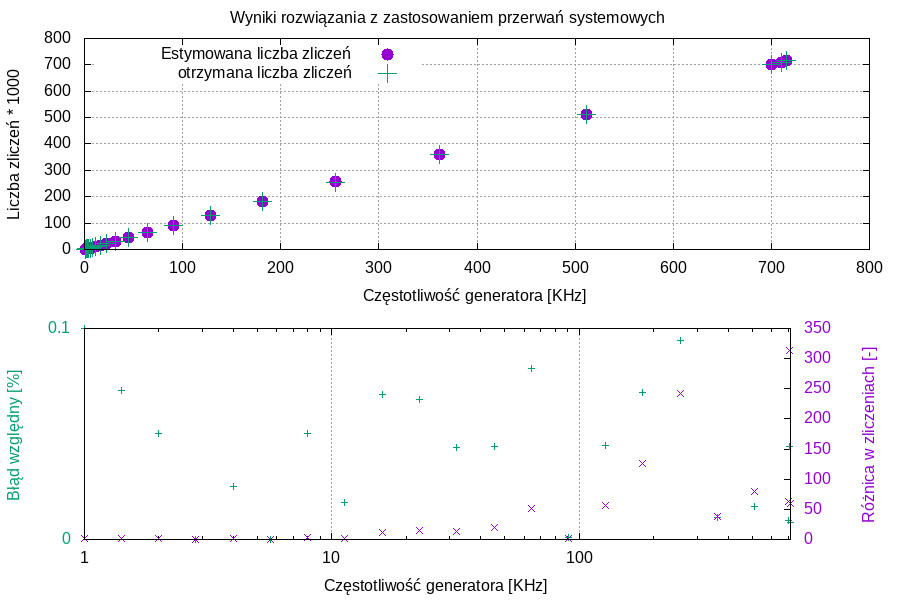
\includegraphics[width=\textwidth]{rts.jpg}
        \caption{Wyniki testów z wykorzystaniem przerwań systemowych}
        \label{rts wyniki}
\end{figure}

\begin{table}
        \centering
        \caption{Wyniki rozwiązania z zastosowaniem przerwań systemowych}
        \label{rts table}
        \begin{tabular}{|c|c|c|c|c|}  
                \hline 
                Częstotliwość [kHz] & Estymowana ilość & Otrzymana ilość & Różnica  & Błąd względny [\%]\\ 
                &  zliczeń &  zliczeń & w zliczeniach & \\ \hline
                1 & 1000 & 1001 & 1 & 0.1000\\ \hline 
                1.414 & 1414 & 1415 & 1 & 0.0707\\ \hline 
                2 & 2000 & 2001 & 1 & 0.0500\\ \hline 
                2.82 & 2820 & 2820 & 0 & 0.0000\\ \hline 
                4 & 4000 & 3999 & 1 & 0.0250\\ \hline 
                5.65 & 5650 & 5650 & 0 & 0.0000\\ \hline 
                8 & 8000 & 7996 & 4 & 0.0500\\ \hline 
                11.3 & 11300 & 11298 & 2 & 0.0177\\ \hline 
                16 & 16000 & 15989 & 11 & 0.0688\\ \hline 
                22.62 & 22620 & 22605 & 15 & 0.0663\\ \hline 
                32 & 32000 & 31986 & 14 & 0.0438\\ \hline 
                45.25 & 45250 & 45230 & 20 & 0.0442\\ \hline 
                64 & 64000 & 63948 & 52 & 0.0813\\ \hline 
                90.5 & 90500 & 90499 & 1 & 0.0011\\ \hline 
                128 & 128000 & 127943 & 57 & 0.0445\\ \hline 
                181 & 181000 & 180874 & 126 & 0.0696\\ \hline 
                256 & 256000 & 255758 & 242 & 0.0945\\ \hline 
                362 & 362000 & 361962 & 38 & 0.0105\\ \hline 
                512 & 512000 & 511920 & 80 & 0.0156\\ \hline 
                700 & 700000 & 699937 & 63 & 0.0090\\ \hline 
                710 & 710000 & 709686 & 314 & 0.0442\\ \hline 
                715 & 715000 & 714941 & 59 & 0.0083\\ \hline
        \end{tabular}
\end{table}

Wyniki pokazują dokładność mieszczącą się w  1\textperthousand, 
jednak błąd w otrzymanym wyniku zależy od częstotliwości generowanych zliczeń.
Może to być spowodowane interferencją przerwania powodującego zliczenie z innymi przerwaniami wymaganymi do działania mikrokontrolera.

Po osiągnięciu częstotliwości granicznej > 0.715 [MHz] program mikrokontrolera przestaje wysyłać dane na komputer zewnętrzny.
Jest to spowodowane tym że zaraz po wyjściu z obsługi przerwania systemowego program natychmiast zaczyna obsługę następnego przerwania. 
Liczba graniczna pozwala przybliżyć czas konieczny na wykonanie jednego przerwania na podstawie przekształcenia wzoru \ref{Cykli w sec}. 
$$ t_p = \frac{1}{f_p} = \sim 1.3986 [\mu s] $$
$$ N_c = \frac{t_p}{t_c} =  \frac{1.3986 \mu s}{11.9 ns} =\sim 118$$
gdzie: \\
        \indent $t_p$ -  czas potrzebny na obsługą przerwania\\
        \indent $t_c$ -  czas jednego cyklu procesora (dział \ref{dzial arduino} ) \\
        \indent $f_p$ -  częstotliwość graniczna przerwań \\
        \indent $N_c$ -  ilość cykli koniecznych na pojedyncze przerwanie \\

Liczba cykli na przerwanie jest mniejsza niż ta szacowana w dziale \ref{dzial arduino} (355 + 128)\cite{ard_opt_git}, wynika to z faktu że poprzednia estymacja była wykonana dla najgorszego przypadku dla nieoptymalizowanego kodu.
Mimo lepszych osiągów niż te szacowane wynik ten nadal odbiega od optymalnego czasu wywołania przerwania (12 + 10) \cite{interupt latency} i wciąż jest znacznie poniżej wymagań projektu. 

Dodatkowe testy potwierdziły że wraz z zwiększeniem ilości badanych kanałów częstotliwość graniczna zmniejsza się jak $\frac{1}{n}$ gdy $n$ to ilość badanych kanałów. 

\subsection{Rozwiązanie z układem zewnętrznych liczników buforujących}

Dane do poniższych wyników zostały uzyskane przez analizę plików archiwalnych otrzymywanych przy działaniu programu do kontroli układu.
Pliki te są przechowywane w formacie JSON.

Analiza sygnałów na oscyloskopie została dokonana na oscyloskopie keysight 3024A. Generator sygnałów używany w układzie badawczym to generator tektonix AFG3102.

Sygnał używany do symulowania impulsów układu RXHDR\_v1 miał wartości 1.8V pick to pick, kształt prostokątny impuls o szerokości 50 us .


\subsubsection{Kalibracja układu}
\label{section kaliblracja}

Przed przystąpieniem do końcowych testów układu konieczne jest przeprowadzenie kalibracji ze względu na uzyskiwany czas martwy układu. 
Oczekiwanym efektem jest regulacja czasu akwizycji w taki sposób że liczba zliczeń będzie odpowiadać ilości impulsów która powinna być uzyskana w czasie akwizycji przez układ bez czasu martwego. 

Zbadano okres jednego cyklu pomiaru (8 kanałów) i uzyskano czas cyklu równy $4.52 \mu s$. Taki cykl jest widoczny na rysunku \ref{Oscyloskop}.
Na podstawie czasu liczby można wyliczyć ilość cykli przypadających na pojedyńcza mikrosekundę.

\begin{equation}
        \label{per cykl}
        CIRCLES\_FOR\_1MS = \frac{1*10^{-3}}{4.52 * 10^{-6}} = 221.238938053
\end{equation}

Korzystając z tej wartości i wartości współczynnika korekcji czasu martwego równego 1 przeprowadzono badania zależności częstotliwości podawanej z generatora do częstotliwości zliczeń dla różnych czasów akwizycji.  

Układ badawczy składał się z komputera, Arduino due, badanego układu elektronicznego, taśmy transmisyjnej, oscyloskopu, generatora impulsów, zasilacza. 

Przeprowadzono trzy badania dla 10 częstotliwości dla 2 czasów akwizycji. Na podstawie tych danych przeprowadzono fitowanie krzywej $f(x) = a*x$ wyniki fitowania umieszczone zostały w tabeli poniżej.

\begin{table}
        \caption{Wyniki fitowania konieczne dla ustalenia korekcji czasu martwego}
        \label{dead time fit}
        \centering
        \begin{tabular}{|c|c|c|c|c|}
                \hline
                Nazwa kanału & czas akwizycji & $a$ & $\Delta a$ & konwersja na 1s \\ \hline
                1A6 & 1000 ms & 0.879395 & $1.893 * 10^{-5}$ & 0.879395 \\ \hline
                2A5 & 500 ms & 0.440366 & $8.156 * 10^{-6}$ & 0.880732 \\ \hline
                2A7 & 500 ms & 0.440352 & $7.939 * 10^{-6}$ & 0.880704 \\ \hline
        \end{tabular}
\end{table}

Na podstawie powyższych danych ustalono wartość współczynnika DEAD\_TIME\_CORECTION równe:
\begin{equation}
        \label{dead time eq}
        DEAD\_TIME\_CORECTION = \frac{1}{\sum^n_i \frac{a_i}{n}} = 1.13636
\end{equation} 

\begin{figure}
        \centering
        \begin{multicols}{2}
                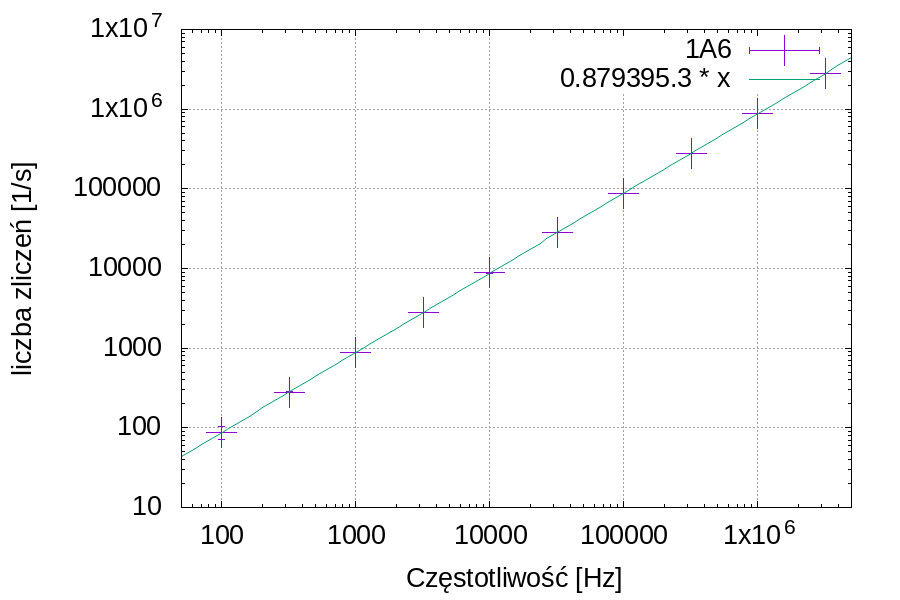
\includegraphics[width=0.5\textwidth]{dead1A6.jpg} \par
                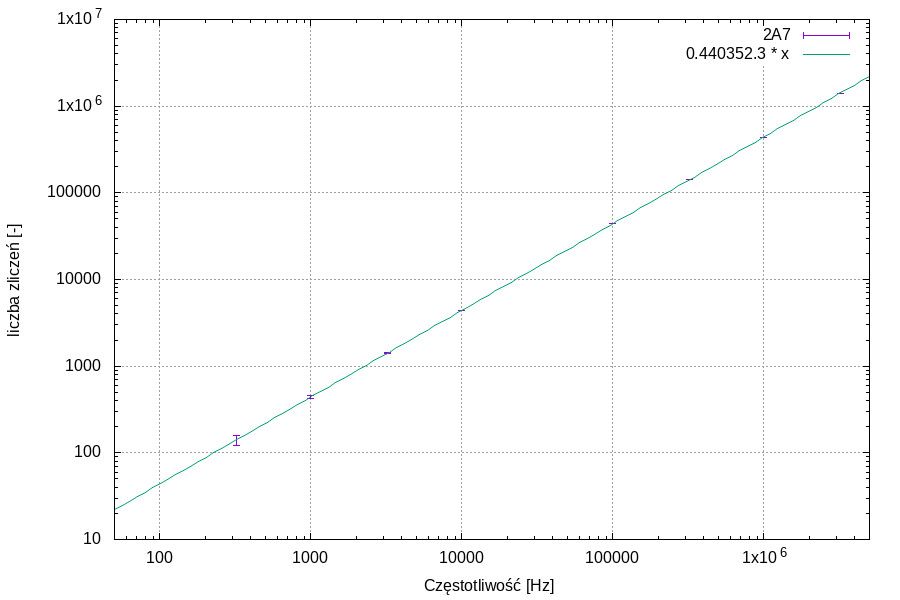
\includegraphics[width=0.5\textwidth]{dead2A7.jpg} \par
        \end{multicols}
        \caption{Wybrane wykresy użyte w celu kalibracji układu}
        \label{wykresy fit calib}
\end{figure}

\subsubsection{Błąd przybliżenia do liczby naturalniej}
Jak widać w fragmencie kodu \ref{code aqw} liczba cykli przeprowadzonych w trakcie pojedyńczej akwizycji musi być liczbą całkowitą. Liczba cykli może być określona wzorem:
\begin{equation}
        N_c [-] = int(A_t*D_t*f_c)
\end{equation}
Gdzie:
\begin{description}
        \item $N_c$ - liczba cykli w procesie akwizycji,
        \item $A_t$ - czas  akwizycji w ms
        \item $D_t$ - współczynnik korekcji czasu martwego 
        \item $f_c$ - ilość cykli w ms
\end{description}

Błąd wprowadzony w wyniku przybliżenia mieści się w przedziale wartości [0,1) pozwala to na wyliczenie maksymalnego względnego błędu uzyskiwanego w wyniku przybliżania:
\begin{equation}
        \Delta N_{c_{max}} [\%] = \frac{1}{A_t*D_t*f_c}  * 100\%
\end{equation} 
Gdzie:
\begin{description}
        \item $\Delta N_{c_{max}}$ - maksymalny względny błąd,
        \item $A_t$ - czas  akwizycji w ms
        \item $D_t$ - współczynnik korekcji czasu martwego 
        \item $f_c$ - ilość cykli w ms
\end{description}

Podstawiając współczynniki uzyskane w dziale \ref{section kaliblracja} możemy uzyskać wartości maksymalnego błędu dla najczęściej używanych czasów akwizycji. Wartości te znajdują się w tabeli \ref{tab przyblizenie niep}. Na podstawie tych wartości można stwierdzić że błąd popełniony podczas przybliżania zmienia się w zależności od czasu akwizycji jest on jednak pomijalnie mały.

\begin{table}
        \centering
        \caption{Wartości błędu wynikające z przybliżenia liczbą całkowitą}
        \label{tab przyblizenie niep}
        \begin{tabular}{|c|c||c|c|}
                \hline
                Czas akwizycji [ms] &   $\Delta N_{c_{max}} [\%]$&Czas akwizycji [ms] &   $\Delta N_{c_{max}} [\%]$ \\ \hline
                50 & 0.007955 & 100 & 0.003977 \\ \hline
                1000 & 0.0003977 & 5000 & 0.00007955 \\ \hline
        \end{tabular}
\end{table}

\subsubsection{Testowanie układu liczników za pomocą generatora zewnętrzego.}

Przy użyciu współczynników otrzymanych w dziale \ref{section kaliblracja} oraz układu badawczego odpowiadającemu temu z działu \ref{section kaliblracja} przeprowadzono test układu z wykorzystaniem dzielnika pozwalającego na dostarczenie sygnałów impulsów, odpowiadającym tym generowanym przez układ RXHDR\_V1, do wszystkich kanałów jednocześnie.
Badanie przeprowadzono dla 10 częstotliwości od 100Hz do 3.2Mhz. Czas akwizycji badania był równy 1s dzięki czemu liczba zliczeń odpowiada liczbie zliczeń. 

\begin{figure}
        \begin{multicols}{2}
            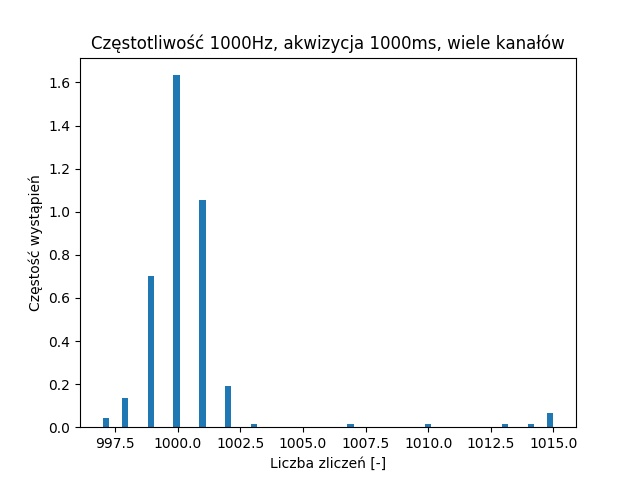
\includegraphics[width=0.5\textwidth]{HM1KHz.jpg} \par    
            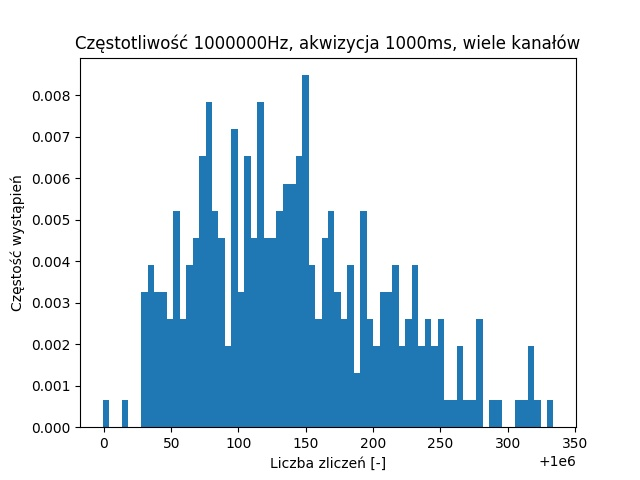
\includegraphics[width=0.5\textwidth]{HM1MHz.jpg} \par    
        \end{multicols} \hfill
        \begin{multicols}{2}
            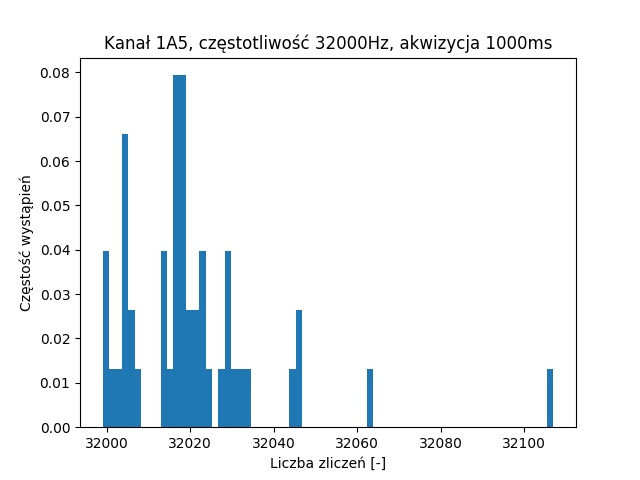
\includegraphics[width=0.5\textwidth]{H1A532KHz.jpg} \par
            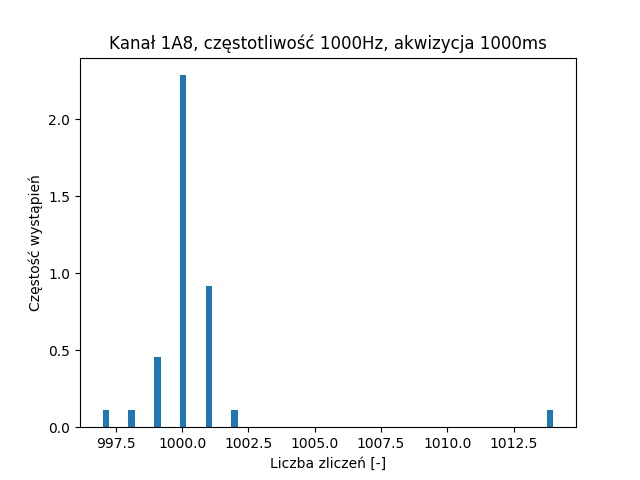
\includegraphics[width=0.5\textwidth]{H1A81KHz.jpg} \par    
        \end{multicols}
        \caption{Histogramy rozrzutu zliczeń dla wybranych kanałów i częstotliwości}
        \label{hist licz}
\end{figure}



Każdy z punktów pomiarowych składał się z serii osobnych akwizycji. Jako wartość punktu pomiarowego ustalono średnią z pomiaru, a jako niepewność pomiaru (zaznaczona na wykresach i uwzględniona w dopasowaniu krzywej) jako odchylenie standardowe średniej. Wartości częstotliwości pojedynczych pomiarów dla wszystkich kanałów dla wybranych częstotliwości znajdują się na histogramach zawartych na rysunkach \ref{hist licz}. 

Wyniki odchylenia standardowego oraz różnicy między podawaną częstotliwością a liczbą zliczeń umieszczone są na rysunku \ref{3d licznik}. Wartości te podawane są jako wartości bezwzględne oraz wartości związane z częstotliwością generowanych sygnałów.

\begin{figure}
        \centering
        \begin{multicols}{2}
                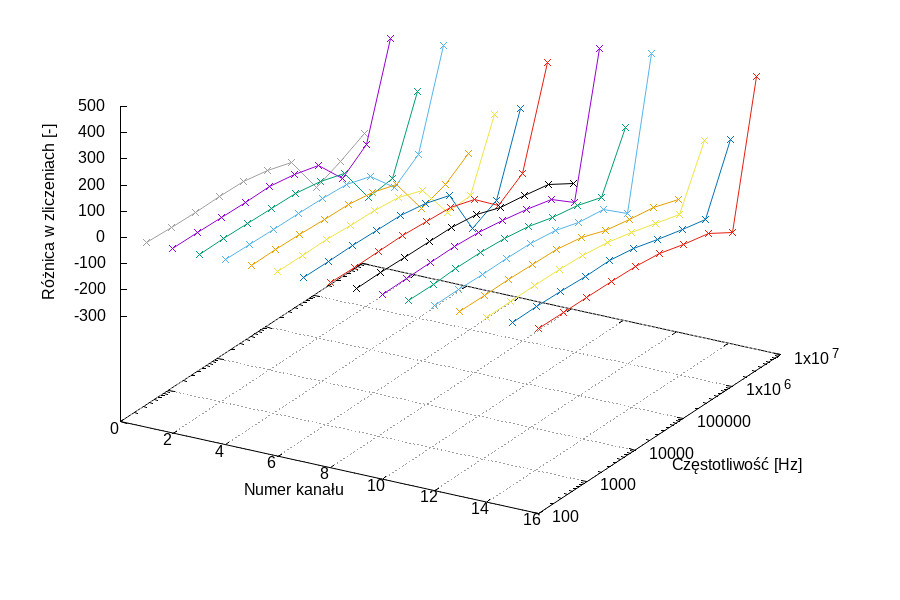
\includegraphics[width=0.5\textwidth]{3d/difLiczik.jpg} \par                
                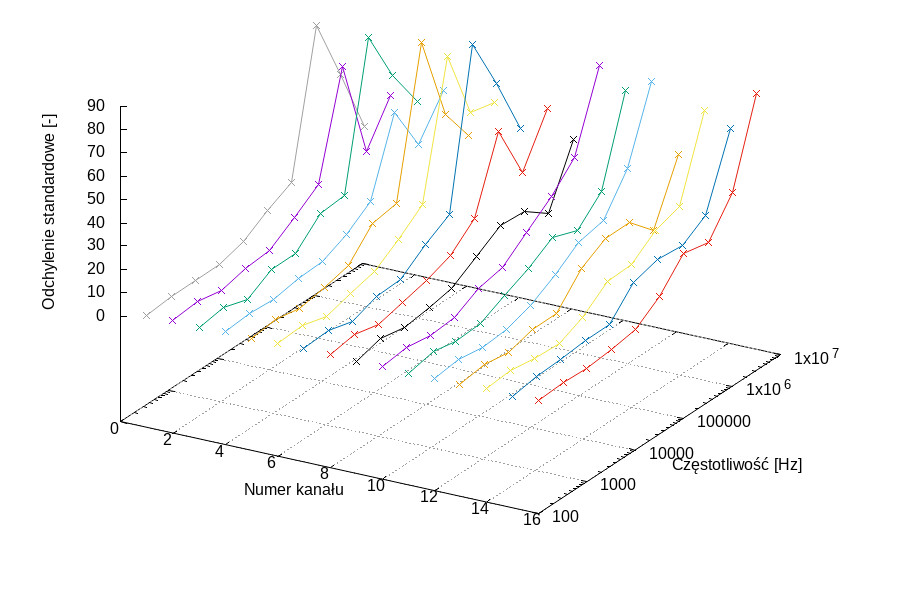
\includegraphics[width=0.5\textwidth]{3d/niepLiczik.jpg} \par                
        \end{multicols} \hfill
        \begin{multicols}{2}
                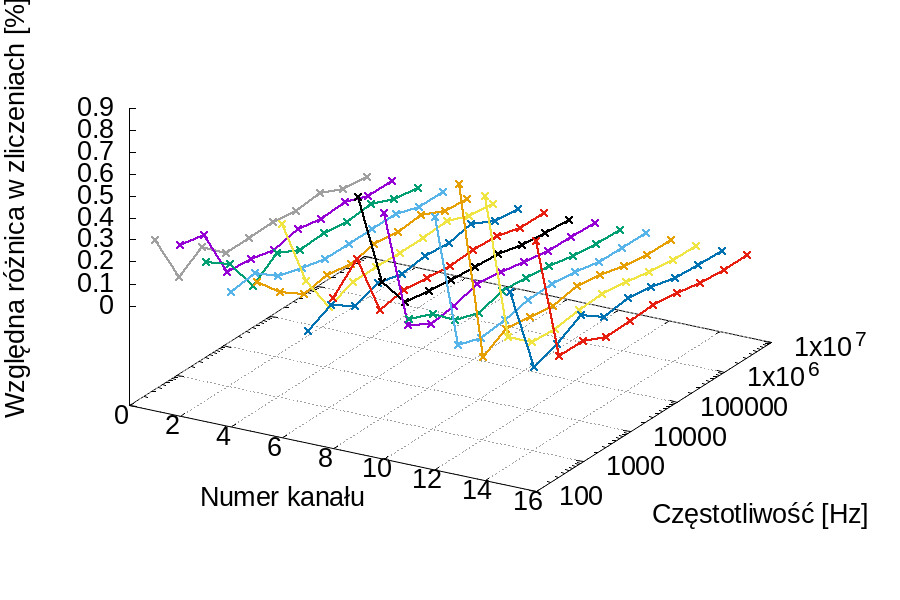
\includegraphics[width=0.5\textwidth]{3d/difWzgLiczik.jpg} \par                
                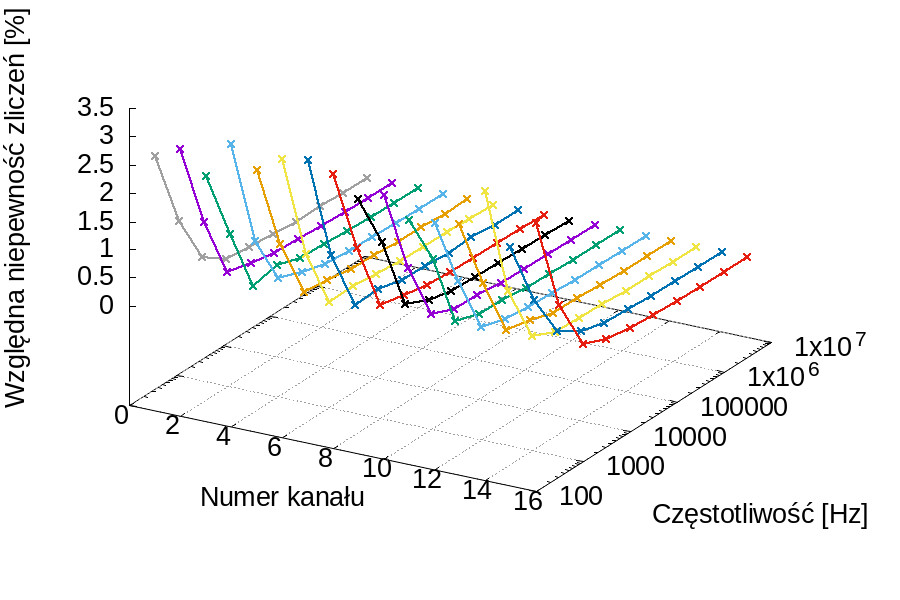
\includegraphics[width=0.5\textwidth]{3d/niepWzgLiczik.jpg} \par                
        \end{multicols}
        \caption{Wartości odchylenia standardowego oraz różnica między zliczeniami podawane w wartościach bezwzględnych oraz jako wartości względne. }
        \label{3d licznik}
\end{figure}

Wybrane wykresy pomiaru zależności częstotliwości od liczby zliczeń umieszczone są na rysunku \ref{multi wyk} a wyniki fitowania znajdują się w tabeli \ref{multi fit}. Wyniki pomiarów fitowane były krzywą $f(x) = a*x$. 
Średnia po wszystkich współczynnikach to $0.999997 \pm 2.56*10^{-5}$
odchylenie standardowe wyników jest równe  $3.94 * 10^{-5}$.

\begin{figure}
        \centering
        \begin{multicols}{2}
                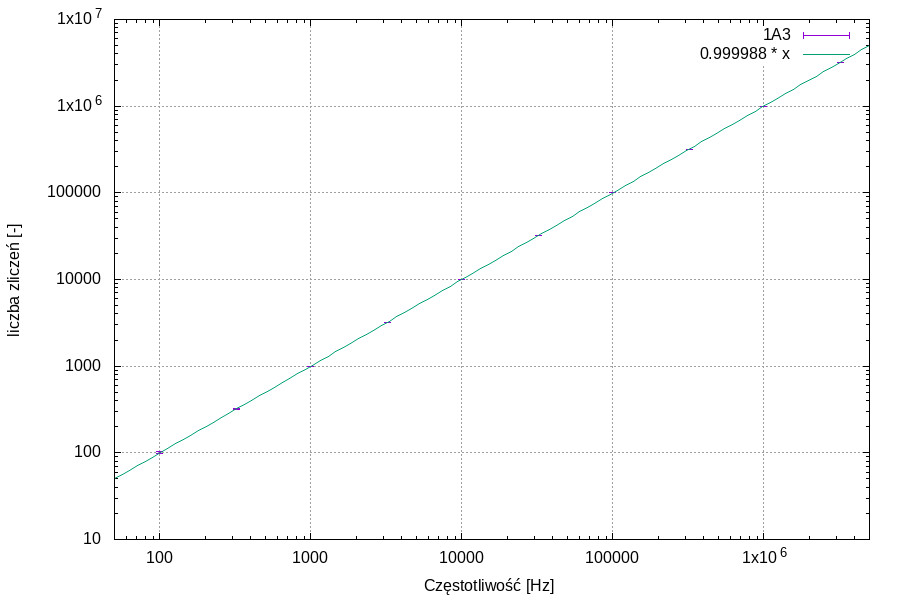
\includegraphics[width=0.5\textwidth]{multi1A3.jpg} \par
                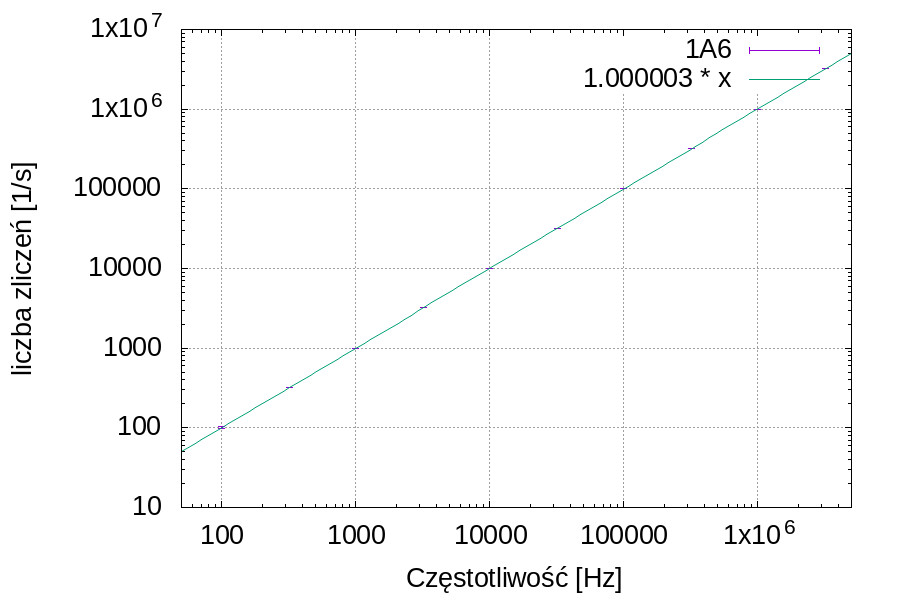
\includegraphics[width=0.5\textwidth]{multi1A6.jpg} \par                
        \end{multicols} \hfill
        \begin{multicols}{2}
                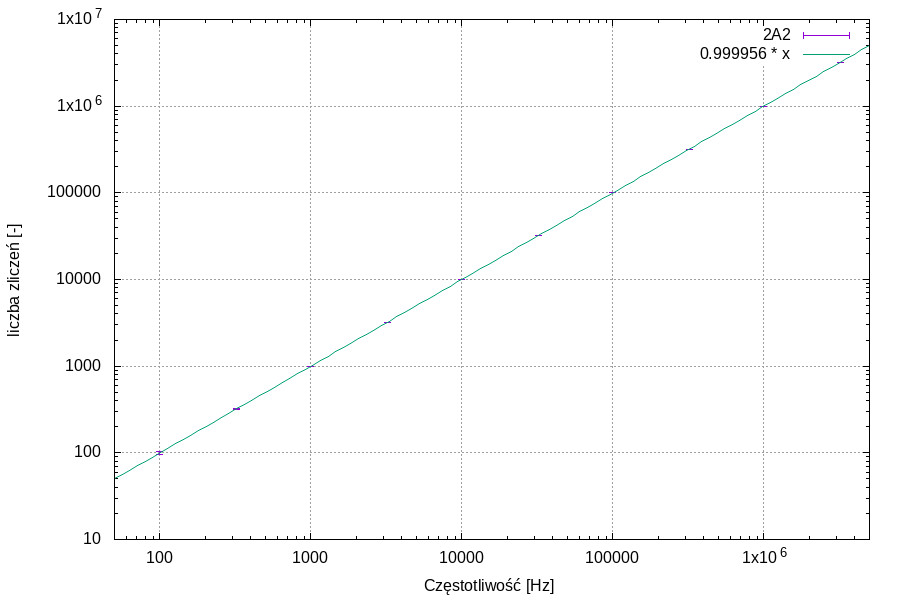
\includegraphics[width=0.5\textwidth]{multi2A2.jpg} \par
                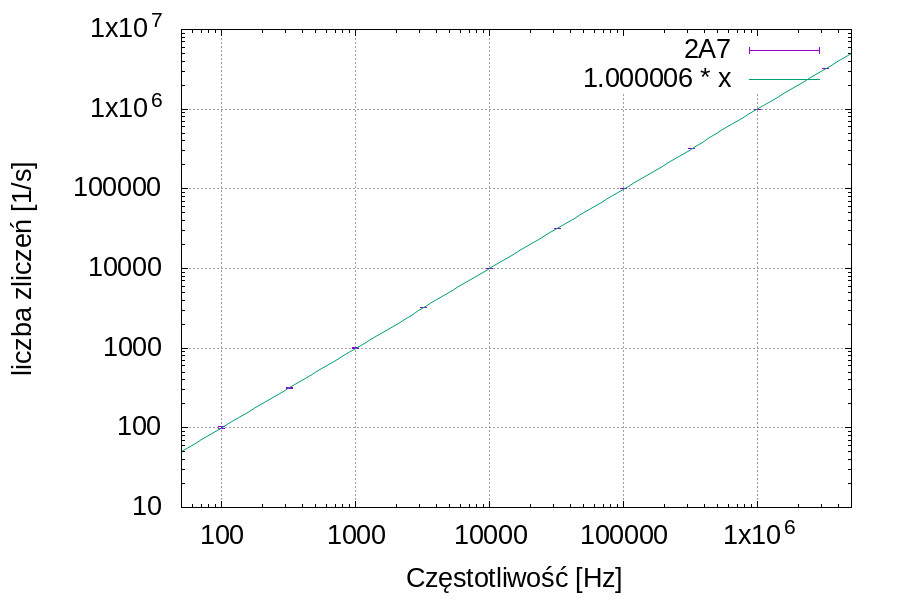
\includegraphics[width=0.5\textwidth]{multi2A7.jpg} \par                
        \end{multicols}
        \caption{Wybrane wykresy testów układu licznika wraz z dopasowanymi krzywymi liniowymi}
        \label{multi wyk}
\end{figure}

\begin{table}
        \centering
        \caption{Wyniki fitowania krzywej $f(x) = a*x$ dla pomiarów generowanych z generatora}
        \label{multi fit}
        \begin{tabular}{|c|c|c||c|c|c|}
                \hline
                kanał & $a$ & $\Delta a$  &kanał & $a$ & $\Delta a$ \\ \hline
                1A1 & 1.00004 & 1.101e-05 & 2A1 &1.00006&1.129e-05 \\ \hline
                1A2 & 0.999961 &2.649e-05& 2A2 &0.999956&4.27e-05 \\ \hline
                1A3 & 0.999988&2.155e-05&2A3 & 1.00003&2.808e-05\\ \hline
                1A4 & 0.999951&2.792e-05&2A4&0.999951&4.309e-05\\ \hline
                1A5&1.00004&1.323e-05&2A5&1.00006&1.223e-05\\ \hline
                1A6&1&2.467e-05&2A6&1.00002&2.792e-05 \\ \hline
                1A7&0.999979&2.002e-05&2A7&1.00001&2.798e-05 \\ \hline
                1A8 &0.999949&2.747e-05&2A8&0.999957&4.373e-05 \\ \hline
        \end{tabular}
\end{table}



\subsubsection{Testowanie układu liczników przy użyciu kanału testowego układu RXHDR\_V1}
\label{section RXHDR test}

Układ badawczy składał się z komputera, Arduino due, badanego układu elektronicznego, taśmy transmisyjnej, oscyloskopu, generatora impulsów, zasilacza, układu RXHDR\_V1, zasilacza wysokiego napięcia. 

Układ RXHDR\_v1 połączony z zestawem liczników buforujących został zasilony napięciem 3.6V oraz 1.8V a detektor został spolaryzowany przez zasilacz wysokiego napięci napięciem 300V. Następnie zestaw ten został połączony z Arduino Due i komputerem kontrolującym. 

Generator połączony z wejściem testowym układu RXHDR\_V1 generował sygnał prostokątny o napięciu ZNAJDŹiWYPEŁNIJ i częstotliwości 100KHz. 

Pomiar polegał na akwizycji danych (1000ms) dla różnych napięć dyskryminatora w celu utworzenia krzywej S. Wykresy tych pomiarów umieszczone zostały na wykresach \ref{s curve test}. Na podstawie tych wykresów przeprowadzono dopasowanie metodą najmniejszych kwadratów krzywej s.

\begin{figure}
        \centering
        \begin{multicols}{2}
                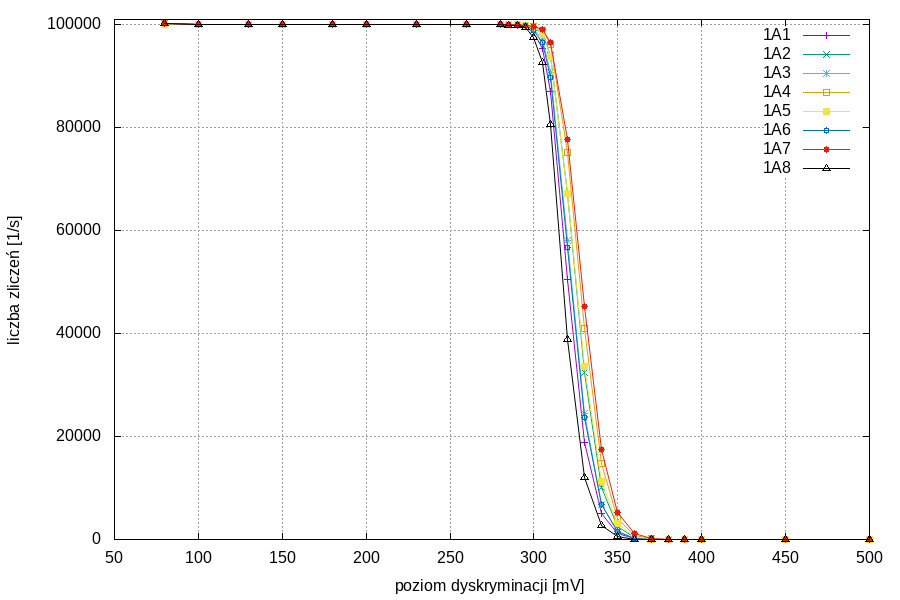
\includegraphics[width=0.5\textwidth]{scurve/test_1A.jpg} \par
                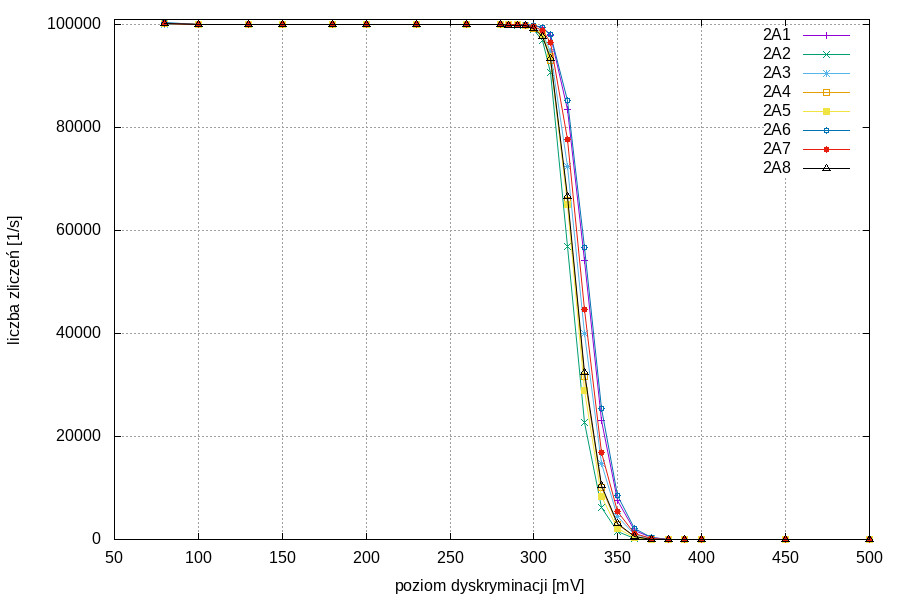
\includegraphics[width=0.5\textwidth]{scurve/test_2A.jpg} \par
        \end{multicols}
        \caption{Krzywe s dla badań z wykorzystaniem sygnałów testowych.}\label{s curve test}
\end{figure}

Funkcja wykorzystana do fitowania krzywej przybrała następującą formę:
\begin{equation}
        \label{test eq}
        S(x) = \frac{f_g}{2} * erf^{-1}(\frac{x-\overline{x}}{\sigma*\sqrt{2}})
\end{equation}
Gdzie:
\begin{description}
        \item $f_g$ - częstotliwość generatora,
        \item $erf^{-1}$ - odwrotna funkcja błędu
        \item $x$ - napięcie dyskryminatora,
        \item $\overline{x}$ - poziom dyskryminacji odpowiadający średniej amplitudzie impulsów (peak position) ,
        \item  $\sigma$ - wartość niepewności odpowiadająca wartości szumowej układu. 
\end{description}

Dopasowywane współczynniki to $f_g$, $\overline{x}$ oraz $\sigma$. Na podstawie wartości $\sigma$ oraz $\overline{x}$ obliczona została wartość ENC. Użyta równość znajduje się poniżej:
\begin{equation}
        ENC [e^-] = \frac{\sigma}{\overline{x}} * \frac{E_{fe}}{E_{(-,+)}}
\end{equation}
Gdzie:
\begin{description}
        \item $ENC$  - równoważny ładunek szumowy,
        \item $E_{(-,+)}$ - energia wymagana na wytworzenie pary dziura/elektron w krzemie,
        \item $\overline{x}$ - poziom dyskryminacji odpowiadający średniej amplitudzie impulsów (peak position) dla źródła ${}^{55}Fe$ (dział \ref{section RXHDR fe})
        \item $E_{fe}$ -  energia deponowana w krzemie przez źródło ${}^{55}Fe$
\end{description}

Wartości tych współczynników znajdują się w tabeli \ref{tabela wsp test} a wykresy tych wartości po kanałach znajdują się na grafice \ref{test fit wsp wyk} 

\begin{figure}
        \begin{multicols}{2}
                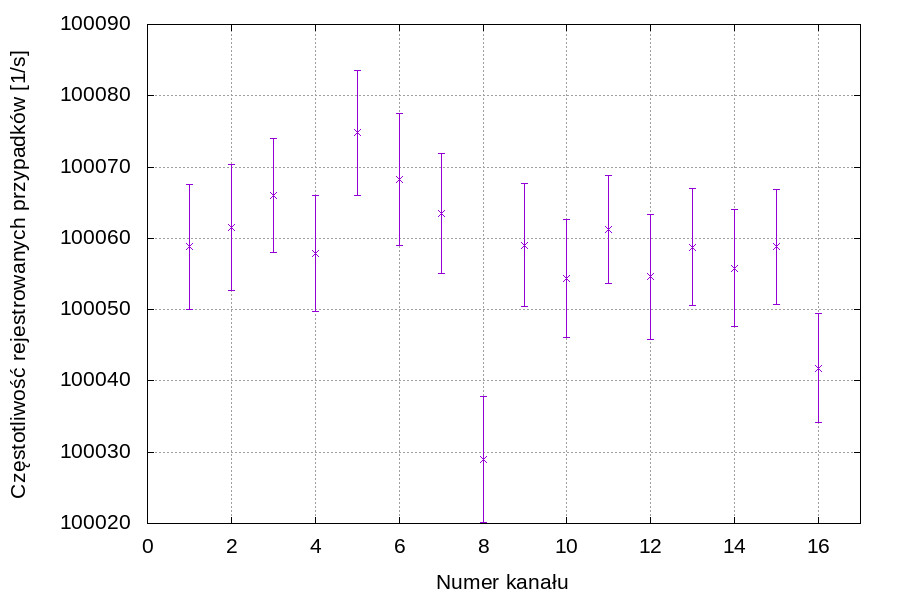
\includegraphics[width=0.5\textwidth]{scurve/Generowana_czestotliwosc_fit.jpg} \par
                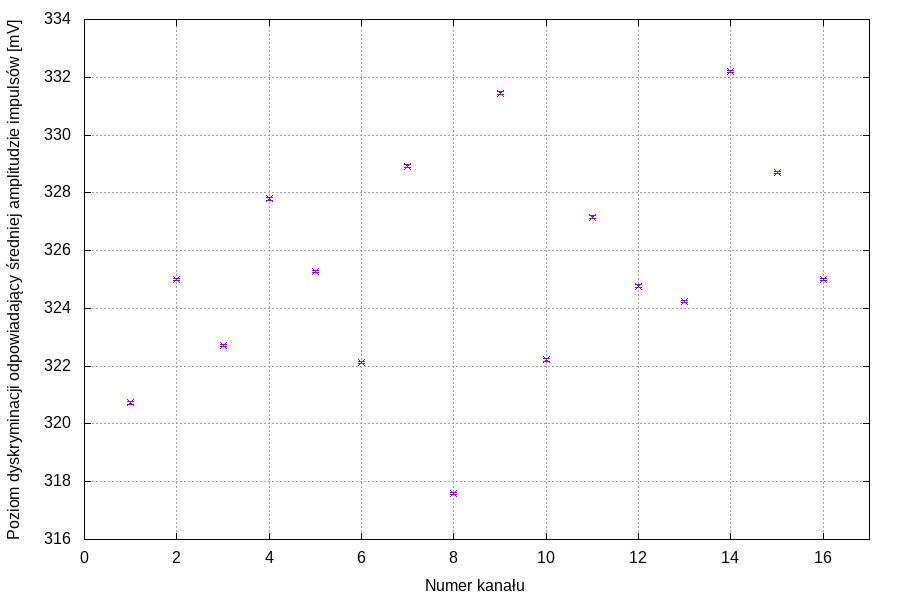
\includegraphics[width=0.5\textwidth]{scurve/srednia_fit.jpg} \par       
        \end{multicols} \hfill
        \begin{multicols}{2}
                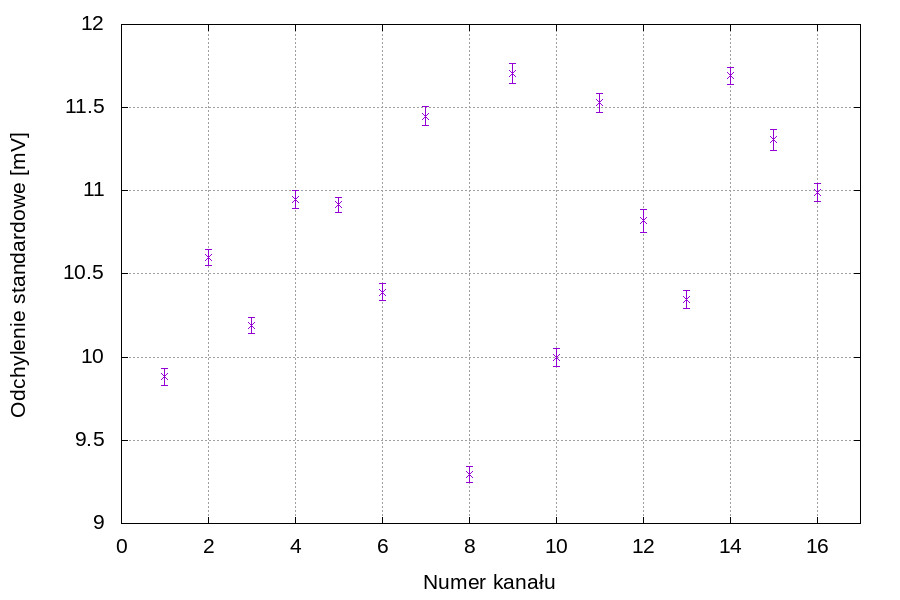
\includegraphics[width=0.5\textwidth]{scurve/odchylenie_fit.jpg} \par
                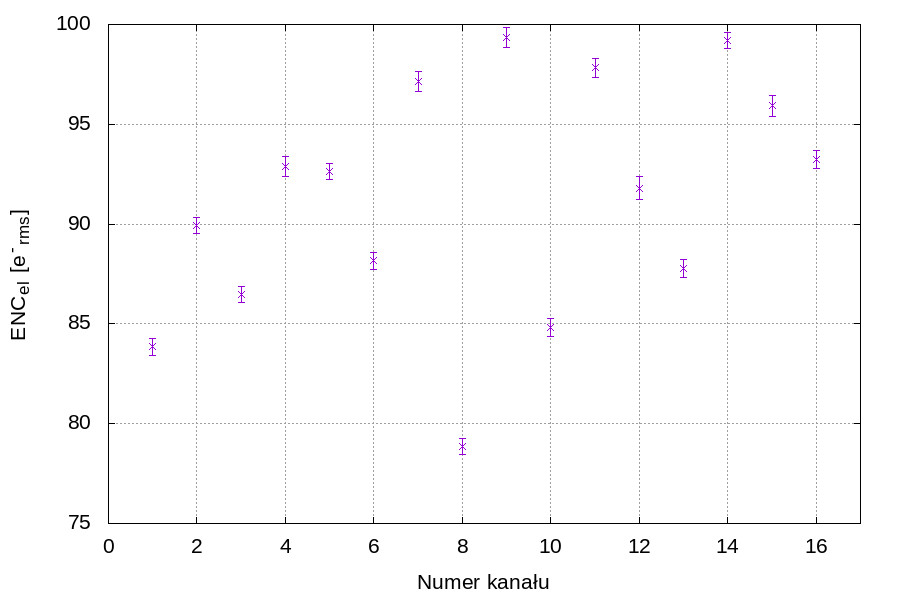
\includegraphics[width=0.5\textwidth]{scurve/ENC_fit_test.jpg} \par
        \end{multicols}
        \caption{Wartości współczynników dopasowanych do krzywych s \ref{s curve test}}
        \label{test fit wsp wyk}
\end{figure}



\begin{table}
        \centering
        \caption{Tabela współczynników testu z użyciem sygnałów testowych, dopasowanych do krzywych s na rysunku \ref{s curve test}}
        \label{tabela wsp test}
        \begin{tabular}{|c|c|c|c|c|c|c|c|c|}
                \hline
                kanał & $f_g$&$\Delta f_g$&$\overline{x}$&$\Delta \overline{x}$&  $\sigma$&  $\Delta \sigma$& ENC & $\Delta$ ENC \\ \hline
                        1A1&100058.81&8.80&320.73&0.06&9.88&0.05&83.84&0.45 \\ \hline 
                        1A2&100061.52&8.83&324.99&0.04&10.60&0.05&89.93&0.42 \\ \hline 
                        1A3&100066.02&7.97&322.72&0.04&10.19&0.05&86.48&0.41 \\ \hline 
                        1A4&100057.83&8.15&327.79&0.05&10.95&0.06&92.89&0.48 \\ \hline 
                        1A5&100074.82&8.80&325.27&0.03&10.92&0.05&92.63&0.39 \\ \hline 
                        1A6&100068.24&9.27&322.14&0.04&10.39&0.05&88.17&0.42 \\ \hline 
                        1A7&100063.50&8.47&328.92&0.05&11.45&0.06&97.14&0.48 \\ \hline 
                        1A8&100028.93&8.85&317.58&0.04&9.30&0.05&78.88&0.40 \\ \hline 
                        2A1&100059.06&8.65&331.45&0.05&11.71&0.06&99.33&0.50 \\ \hline 
                        2A2&100054.34&8.28&322.21&0.05&10.00&0.05&84.84&0.46 \\ \hline 
                        2A3&100061.20&7.59&327.16&0.04&11.53&0.06&97.82&0.49 \\ \hline 
                        2A4&100054.62&8.78&324.77&0.06&10.82&0.07&91.80&0.59 \\ \hline 
                        2A5&100058.74&8.20&324.23&0.04&10.35&0.05&87.79&0.45 \\ \hline 
                        2A6&100055.83&8.27&332.20&0.04&11.69&0.05&99.20&0.42 \\ \hline 
                        2A7&100058.83&8.09&328.71&0.05&11.31&0.06&95.93&0.52 \\ \hline 
                        2A8&100041.80&7.66&325.00&0.04&10.99&0.05&93.25&0.44 \\ \hline                    
        \end{tabular}
\end{table}


\subsubsection{Testowanie układu liczników przy układu RXHDR\_V1 oraz żródła promieniotwórczego}
\label{section RXHDR fe}

Przeprowadzono badanie analogicznie do tych w dziale \ref{section RXHDR test}, jednak zamiast impulsów wprowadzanych na wejście testowe układu RXHDR\_V1 sygnał generowany był przez źródło promieniotwórcze ${}^{55}fe$ ustawione bezpośrednio nad oknem detektora. 

Wykresy zależności napięcia dyskryminatora względem liczby zliczeń umieszczone zostały na wykresie \ref{s curve fe}. 

\begin{figure}[]
        \centering
        \begin{multicols}{2}
                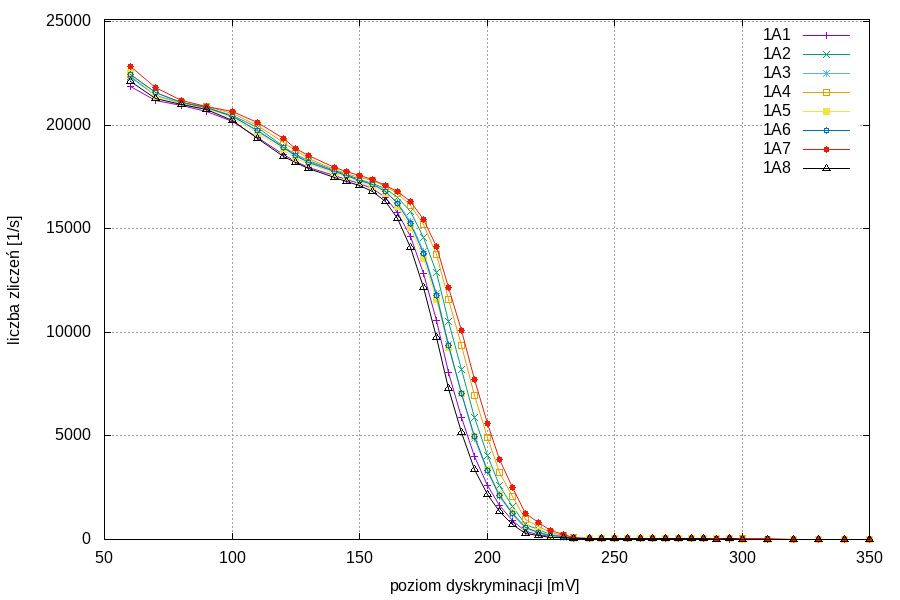
\includegraphics[width=0.5\textwidth]{scurve/fe_1A.jpg} \par
                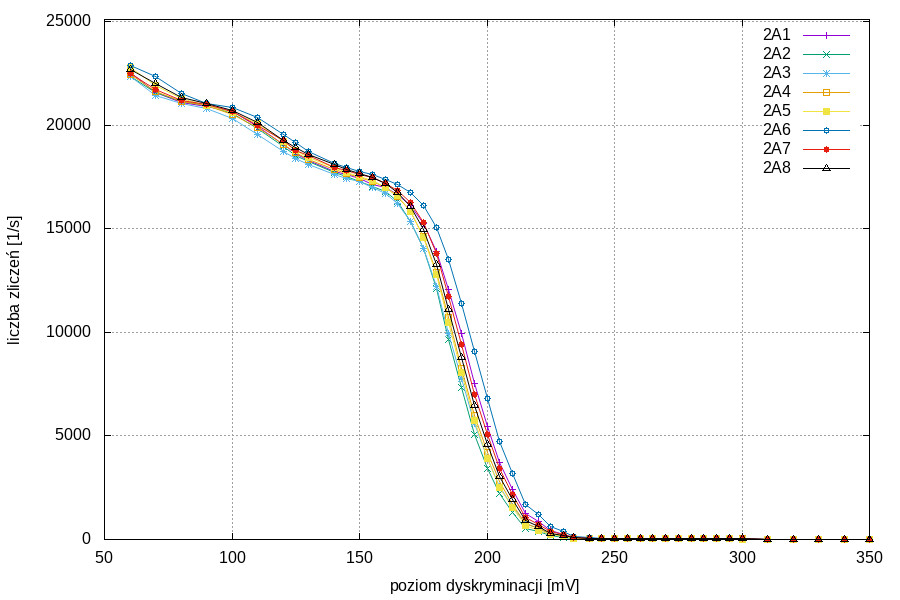
\includegraphics[width=0.5\textwidth]{scurve/fe_2A.jpg} \par
                
        \end{multicols}
        \caption{Krzywe s dla badań z wykorzystaniem źródła promieniotwórczego}
        \label{s curve fe}
\end{figure}

Do wykresów na rysunku \ref{s curve fe} dopasowana została krzywa s z uwzględnieniem współczynnika podziału ładunku. Wzór przybiera następującą postać:

\begin{equation}
        \label{test eq}
        S(x) = (1-RCS * (\frac{x}{\overline{x}}-0.5)) * \frac{f_g}{2} * erf^{-1}(\frac{x-\overline{x}}{\sigma*\sqrt{2}})
\end{equation}
Gdzie:
\begin{description}
        \item $f_g$ - częstotliwość generatora,
        \item $erf^{-1}$ - odwrotna funkcja błędu
        \item $x$ - napięcie dyskryminatora,
        \item $\overline{x}$ - poziom dyskryminacji odpowiadający średniej amplitudzie impulsów (peak position) ,
        \item  $\sigma$ - wartość niepewności odpowiadająca wartości szumowej układu,
        \item $RCS$ -  współczynnik podziału ładunku.
\end{description}

Na podstawie wartości $\sigma$ oraz $\overline{x}$ wyliczona została wartość ENC:

\begin{equation}
        ENC [e^-] = \frac{\sigma}{\overline{x}} * \frac{E_{fe}}{E_{(-,+)}}
\end{equation}
Gdzie:
\begin{description}
        \item $ENC$  - równoważny ładunek szumowy,
        \item $E_{(-,+)}$ - energia wymagana na wytworzenie pary dziura/elektron w krzemie,
        \item $\overline{x}$ - poziom dyskryminacji odpowiadający średniej amplitudzie impulsów (peak position) dla fitowanego kanału,
        \item $E_{fe}$ -  energia deponowana w krzemie przez źródło ${}^{55}Fe$
\end{description}

Wartości otrzymanych współczynników wraz z niepewnościami umieszczone zostały w tabeli \ref{tabela wsp fe}. Wykresy wartości tych współczynników po kanałach znajdują się na rysunku \ref{wyk wsp fe}.

Średnia wartość $\overline{x}$ dla wszystkich kanałów została policzona i wynosi $191.02 \pm 0.17 [mV]$


\begin{table}
        \centering
        \caption{Tabela współczynników testu z użyciem źródła promieniotwórczego, dopasowanych do krzywych s na rysunku \ref{s curve fe}}
        \label{tabela wsp fe}
        \begin{tabular}{|c|c|c|c|c|c|c|c|c|c|c|}
        \hline
        kanał & $f_g$&$\Delta f_g$&$\overline{x}$&$\Delta \overline{x}$&  $\sigma$&  $\Delta \sigma$ &RCS&$\Delta$ RCS& ENC & $\Delta$ ENC \\ \hline
        1A1&20173.65&52.14&185.81&0.17&15.14&0.14&0.44&0.01&132.10&1.27  \\ \hline 
        1A2&20344.09&51.38&191.21&0.16&14.82&0.14&0.47&0.01&125.65&1.19  \\ \hline 
        1A3&20403.52&45.63&188.55&0.15&15.27&0.13&0.45&0.01&131.27&1.11  \\ \hline 
        1A4&20379.81&43.01&193.48&0.16&15.37&0.12&0.46&0.01&128.80&1.01  \\ \hline 
        1A5&20315.39&46.61&188.60&0.19&15.61&0.14&0.47&0.01&134.15&1.19  \\ \hline 
        1A6&20385.95&47.43&188.80&0.18&15.19&0.13&0.47&0.01&130.37&1.12  \\ \hline 
        1A7&20458.17&44.85&195.31&0.17&15.34&0.14&0.49&0.01&127.34&1.17  \\ \hline 
        1A8&20277.88&46.78&184.63&0.20&15.08&0.15&0.47&0.01&132.43&1.30  \\ \hline 
        2A1&20336.26&45.10&195.12&0.17&15.26&0.14&0.50&0.01&126.75&1.17  \\ \hline 
        2A2&20433.52&48.91&189.32&0.19&15.17&0.15&0.47&0.01&129.86&1.26  \\ \hline 
        2A3&20285.03&44.09&190.34&0.19&16.07&0.15&0.48&0.01&136.87&1.26  \\ \hline 
        2A4&20433.73&43.03&191.42&0.18&15.24&0.15&0.47&0.01&129.03&1.32  \\ \hline 
        2A5&20607.82&42.85&190.80&0.17&14.96&0.15&0.48&0.01&127.09&1.25  \\ \hline 
        2A6&20633.18&44.10&198.36&0.17&14.90&0.13&0.49&0.01&121.79&1.04  \\ \hline 
        2A7&20470.14&43.72&193.59&0.16&15.80&0.09&0.46&0.01&132.32&0.77  \\ \hline 
        2A8&20658.61&44.82&192.15&0.17&15.76&0.13&0.47&0.01&132.95&1.07  \\ \hline 

        \end{tabular}
\end{table}

\begin{figure}
        \begin{multicols}{2}
                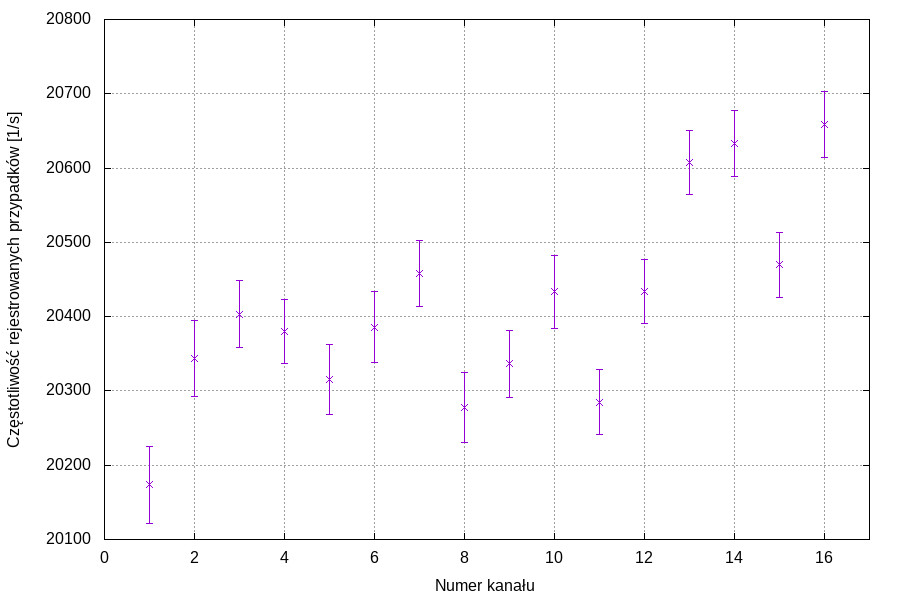
\includegraphics[width=0.5\textwidth]{scurve/Generowana_czestotliwosc_fit_fe.jpg} \par
                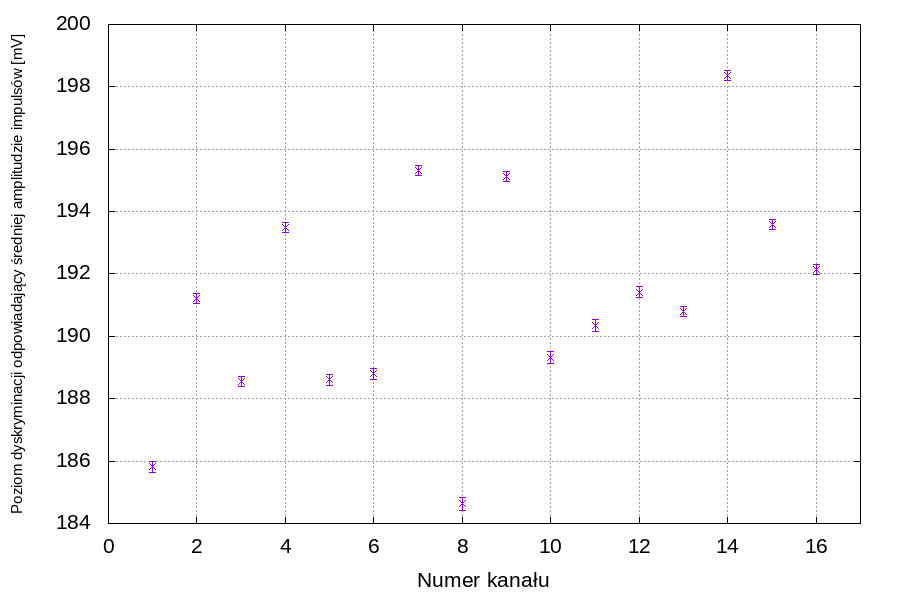
\includegraphics[width=0.5\textwidth]{scurve/srednia_fit_fe.jpg} \par       
        \end{multicols} \hfill
        \begin{multicols}{2}
                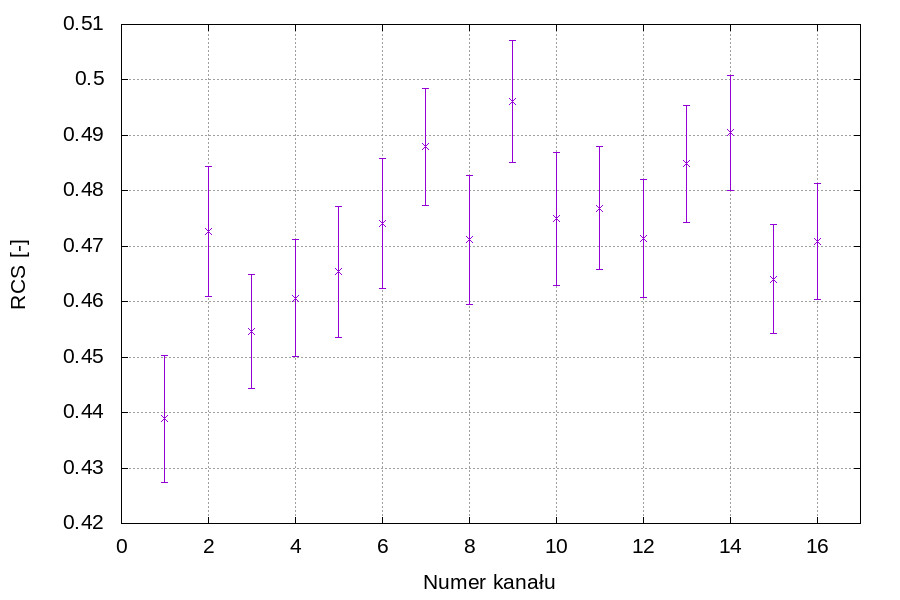
\includegraphics[width=0.5\textwidth]{scurve/RCS_fit_fe.jpg} \par
                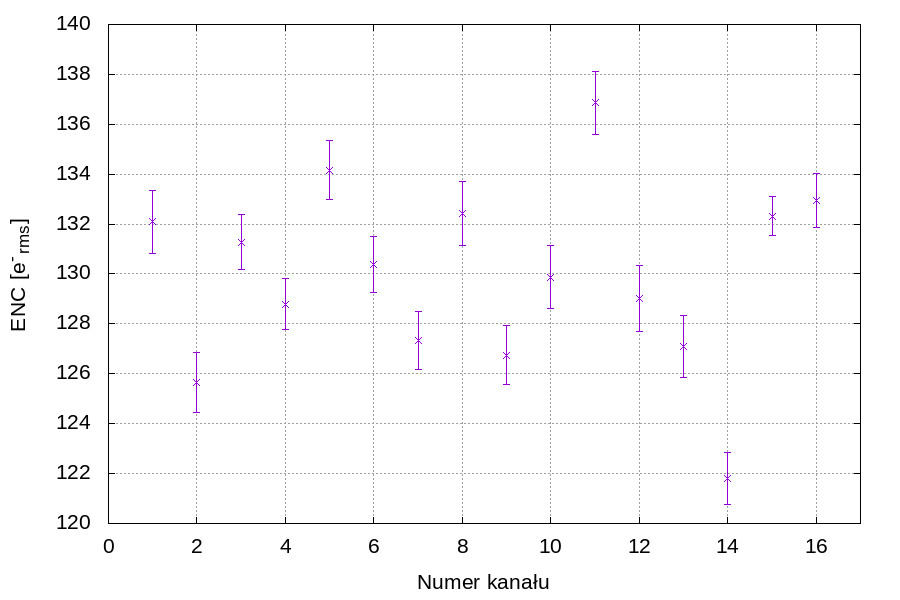
\includegraphics[width=0.5\textwidth]{scurve/ENC_fit_fe.jpg} \par
        \end{multicols}
        \caption{Wartości współczynników dopasowanych do krzywych s \ref{s curve fe}}
        \label{wyk wsp fe}
\end{figure}